%*********************************************************************
%	Experimental Validation
%*********************************************************************
\chapter{Experimental Validation}
\label{ch:Validation}
%---------------------------------------------------------------------
In order to validate the processing pipeline as a whole, two methods are used. Firstly the pipeline is applied to experimental data captured during the characterisation stage of the known relief objects. Whilst this does not acurately describe the sediment surface in situ, it allows for an analytical evaluation the pipeline, whilst providing some resemblance for the true conditions.

Secondly, scans of the surface of sand, taken from the langebaan lagoon, was performed. This was taken for dry, wet and submerged sand, in both flat and shaped forms. This experimentation provides little analytical results, but helps to get a qualitative understanding of the performance in conditions closer to environmental.

\section{Controlled Targets}

\subsection{Process}
The rugosity estimation pipeline is applied to scans taken of reference objects shown in \autoref{Apendix:Reference_Objects}. These scans are re-used from the characterisation process \autoref{ch:experiments}. These scans had the filters identified in \autoref{ch:experiments} applied to them. Cropping and fusion was then applied. This reconstructed surface was then cropped down to just the reference object, and the evaluation was performed on it. The results of which are then compared to the results obtained via analytical evaluation of the reference object file .stl. This provides an analytical comparison between the results of scanning and processing, and the known relief.

\subsection{Results}

Each smooth shape (big egg box and small egg box) were processed using the rugosity\_metrics processing pipeline compared against their respective reference .stl files. The evaluation was performed on both fused and single scan results, and each metric applied all four detrending methods (planar, quadratic, cubic and quartic). These rugosity metrics are shown in \autoref{tab:Big_Egg_Rugosity} and \autoref{tab:Small_Egg_Rugosity}, which are in turn plotted in \autoref{fig:Big-Egg-Rugosity} and \autoref{fig:Small-Egg-Rugosity}.

There are two main points to be discussed with these results. Firstly is the effects of the different detrending results. The results show that planar and quadratic detrending methods tend to produce results that better match the ground truth. Care must be taken here since this analysis applies the same detrend to the ground truth. Thus the planar detrending should be the best representation of the ground truth rugosity. The primary reason for planar and quadraticdetrending giving the best performance can be seen in \autoref{fig:Big-Egg-Rugosity}, where the lower wavelength shape closely alignes with the higher order detrending methods, and thus they tend to remove this information. These can be visually seen in \autoref{Appendix:Validation_Results} where the cubic and quartic detrending methods tend to remove actual shape of the big egg box surface, rather than underlying trends.

Secondly, and most importantly, is that these results are innacuratly representing the truth. The plots show that single scans generally produce rugosity metrics that are more closely aligned with the reernce objects. This is contrary to what is expected, as the fused results generally provide a closer representation to the ground truth. The fundamental reason for this discrepency is actually a misleading result. The reconstrucitons for these reference objects are not completely accurate, and all feature some scale error, and underrepresetnt the amplitude of the reference waveforms. This means that the reconstructions will always report a lower rugosity compare to what the true waveforms have. This is where the inflated single scan performance arives. Since the single scans have a higher depth noise, this noise arteficially increases the roughness of the surface. This can be seen in \autoref{fig:smallwave701mmfusedside} and \autoref{fig:smallwave701mmsingleside}. This arteficial increase in the roughness, results in a higher rugosity, which results in an arteficially better result.


% Generated by rstable 0.1.0 on 2026-10-22T23:40:11
% Figure: /home/joab/Documents/4022/Report/uct-thesis-template/figs/ch7/Shaped/Big_Egg_Rugosity.rsplot.json
% Data:   /home/joab/Documents/4022/Data/roughness_out_V2/Shapes/roughness_results.csv
% Re-open: Big_Egg_Rugosity_table.rstable.json. Needs booktabs and makecell.
\begin{table}[ht]
	\centering
	\small
	\setlength{\tabcolsep}{8pt}
	\caption{Each value is over n = 1 rows.}
	\label{tab:Big_Egg_Rugosity}
	\begin{tabular}{l l c c}
		\toprule
		Detrend Method & Scan & \makecell{Rugosity\\{\footnotesize mean $\pm$ SD}} & \makecell{Ref rugosity\\{\footnotesize mean $\pm$ SD}} \\
		\midrule
		cubic & Big Egg Box Fused & 1.19 & 1.27 \\
		 & Big Egg Box Single & 1.26 & 1.26 \\
		\addlinespace
		planar & Big Egg Box Fused & 1.25 & 1.34 \\
		 & Big Egg Box Single & 1.31 & 1.34 \\
		\addlinespace
		quadratic & Big Egg Box Fused & 1.25 & 1.34 \\
		 & Big Egg Box Single & 1.31 & 1.34 \\
		\addlinespace
		quartic & Big Egg Box Fused & 1.19 & 1.27 \\
		 & Big Egg Box Single & 1.26 & 1.26 \\
		\bottomrule
	\end{tabular}
\end{table}


% Generated by rstable 0.1.0 on 2026-10-22T23:40:54
% Figure: /home/joab/Documents/4022/Report/uct-thesis-template/figs/ch7/Shaped/Small_Egg_Rugosity.rsplot.json
% Data:   /home/joab/Documents/4022/Data/roughness_out_V2/Shapes/roughness_results.csv
% Re-open: Small_Egg_Rugosity_table.rstable.json. Needs booktabs and makecell.
\begin{table}[ht]
	\centering
	\small
	\setlength{\tabcolsep}{8pt}
	\caption{Fused and Single Scan Rugosity Measurements for Small Egg Box Surface.}
	\label{tab:Small_Egg_Rugosity}
	\begin{tabular}{l l c c}
		\toprule
		Detrend Method & Scan & \makecell{Rugosity\\{\footnotesize mean}} & \makecell{Ref rugosity\\{\footnotesize mean}} \\
		\midrule
		cubic & Small Egg Box Fused & 1.26 & 1.69 \\
		 & Small Egg Box Single & 1.31 & 1.69 \\
		\addlinespace
		planar & Small Egg Box Fused & 1.26 & 1.69 \\
		 & Small Egg Box Single & 1.31 & 1.69 \\
		\addlinespace
		quadratic & Small Egg Box Fused & 1.26 & 1.69 \\
		 & Small Egg Box Single & 1.31 & 1.69 \\
		\addlinespace
		quartic & Small Egg Box Fused & 1.25 & 1.69 \\
		 & Small Egg Box Single & 1.31 & 1.69 \\
		\bottomrule
	\end{tabular}
\end{table}


\begin{figure}[htbp]
	\centering
	\begin{subfigure}[t]{0.5072\textwidth}
		\centering
		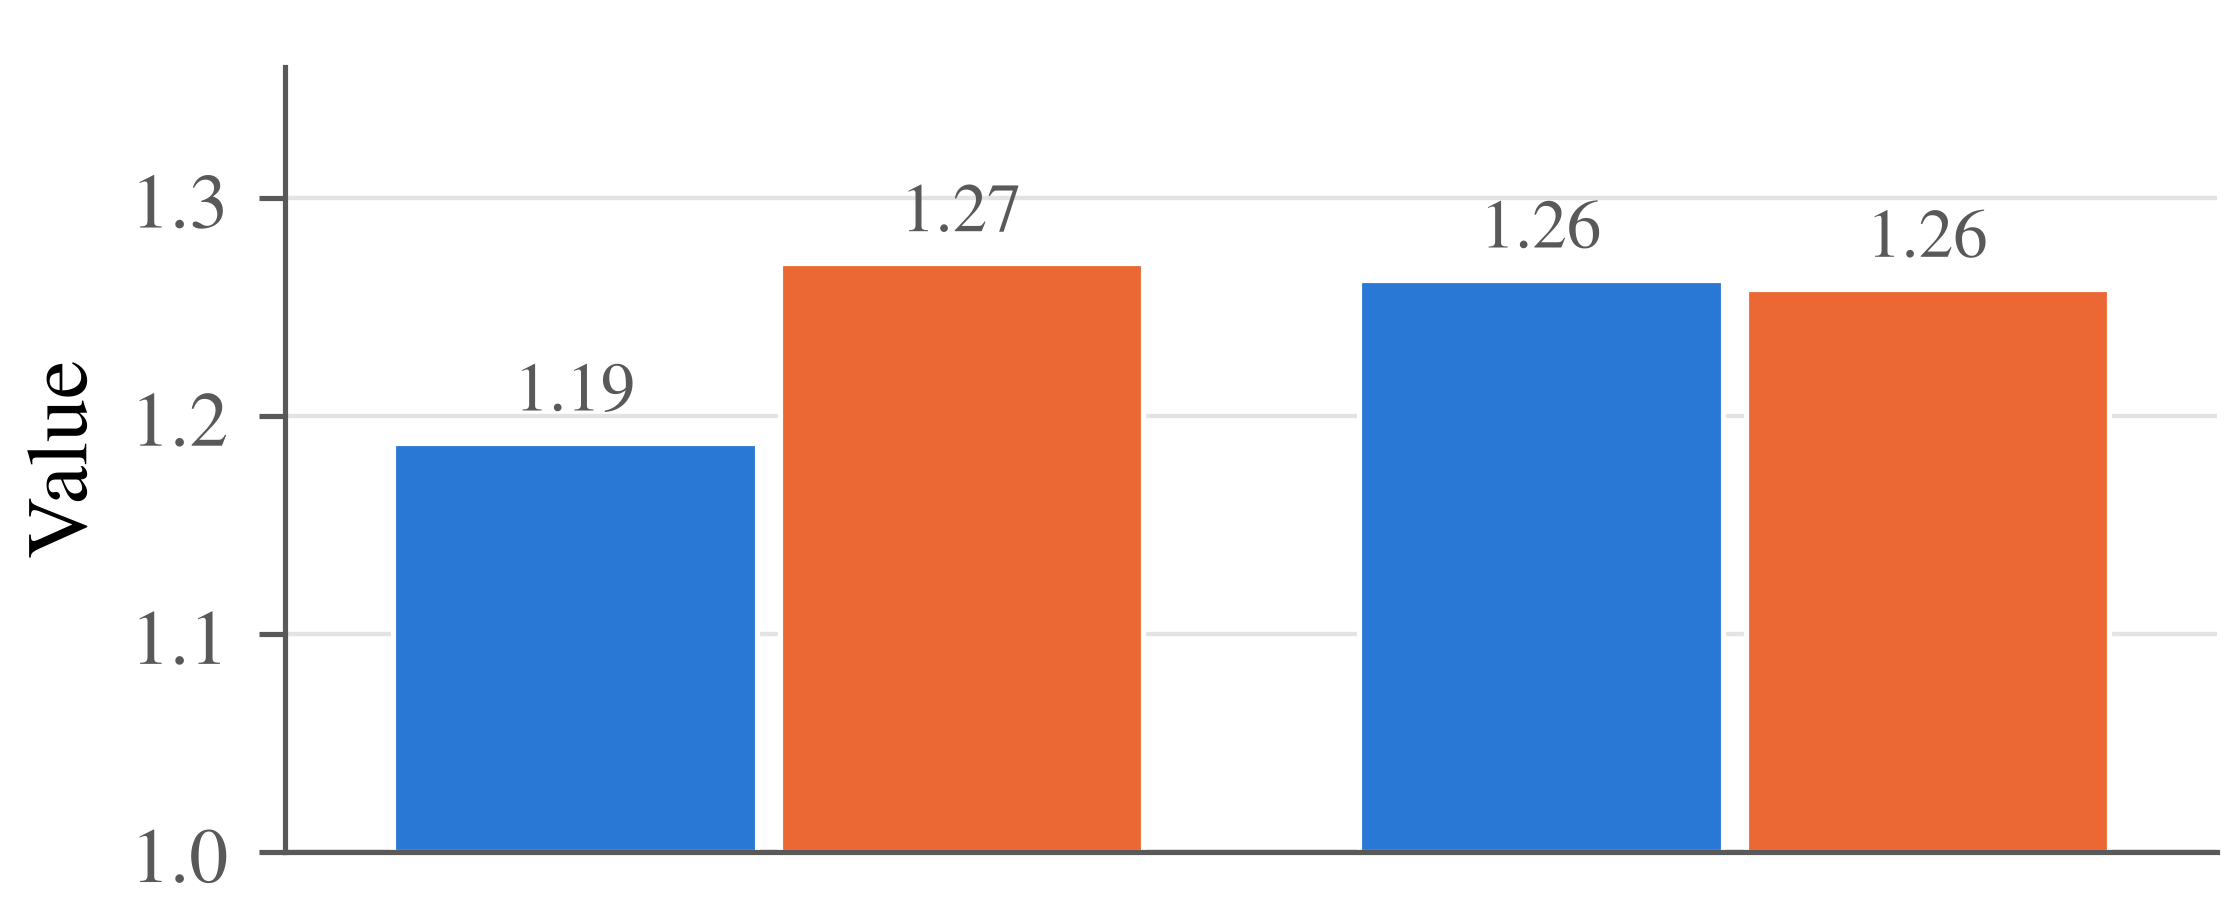
\includegraphics[width=\linewidth]{figs/ch7/Shaped/Big_Egg_Rugosity_p1}
		\caption{cubic}
		\label{fig:Big-Egg-Rugosity-1}
	\end{subfigure}\hfill
	\begin{subfigure}[t]{0.4528\textwidth}
		\centering
		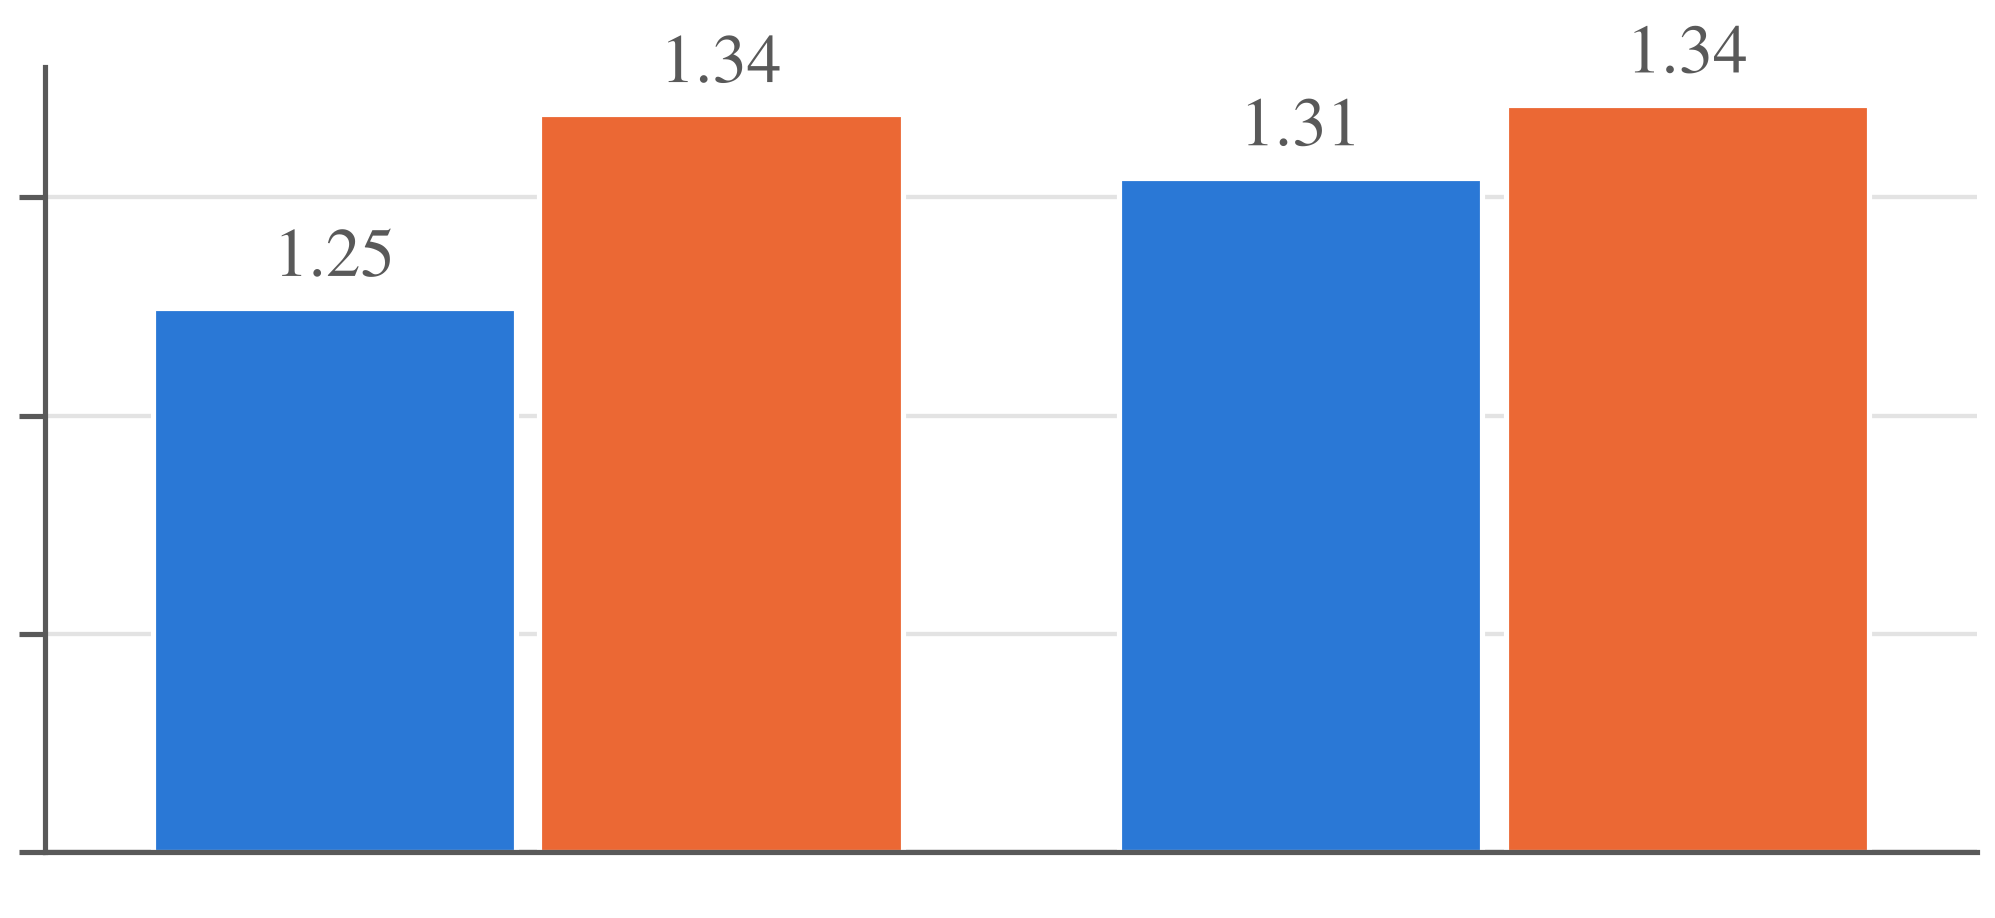
\includegraphics[width=\linewidth]{figs/ch7/Shaped/Big_Egg_Rugosity_p2}
		\caption{planar}
		\label{fig:Big-Egg-Rugosity-2}
	\end{subfigure}
	\par\medskip
	\begin{subfigure}[t]{0.5072\textwidth}
		\centering
		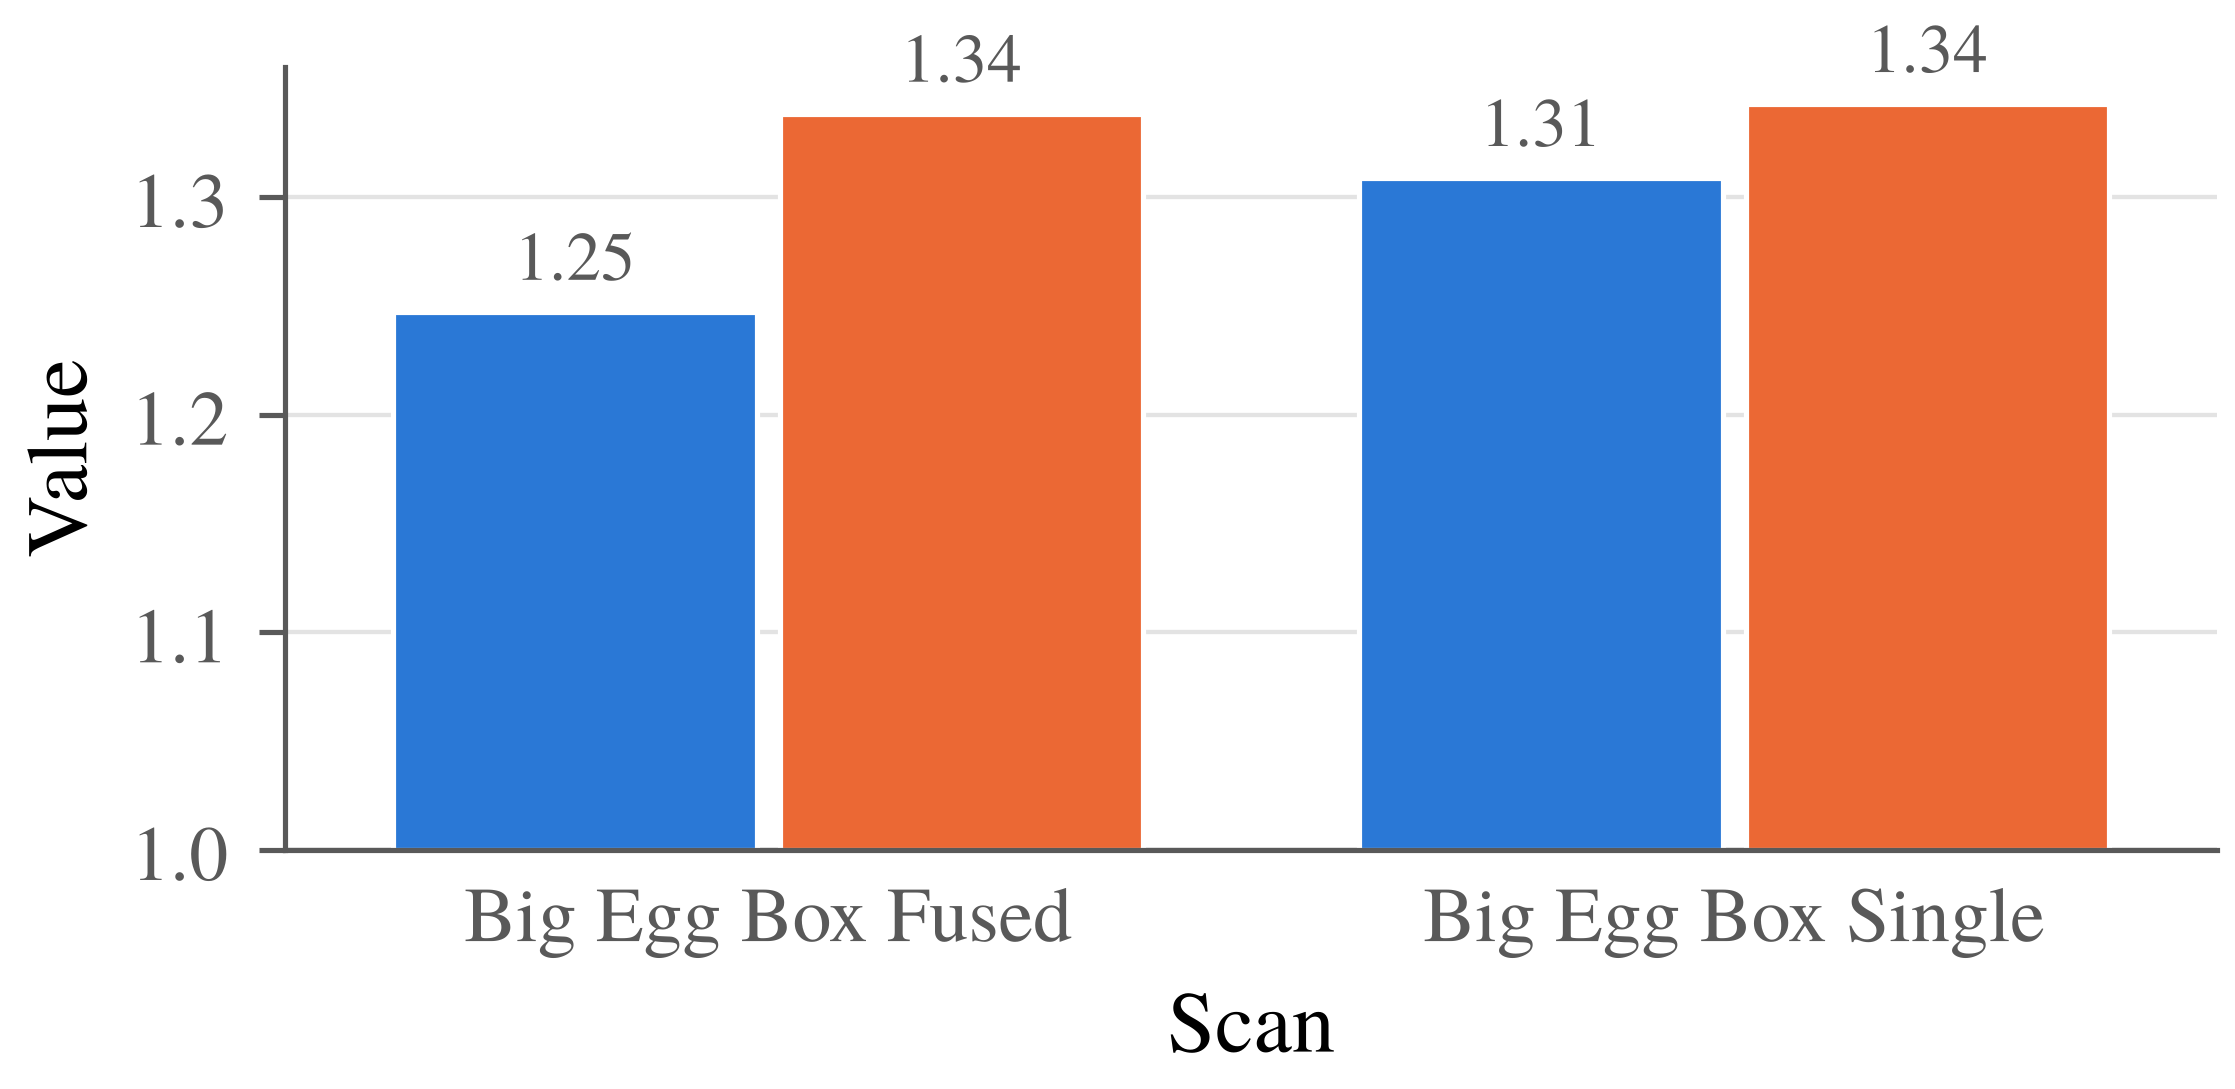
\includegraphics[width=\linewidth]{figs/ch7/Shaped/Big_Egg_Rugosity_p3}
		\caption{quadratic}
		\label{fig:Big-Egg-Rugosity-3}
	\end{subfigure}\hfill
	\begin{subfigure}[t]{0.4528\textwidth}
		\centering
		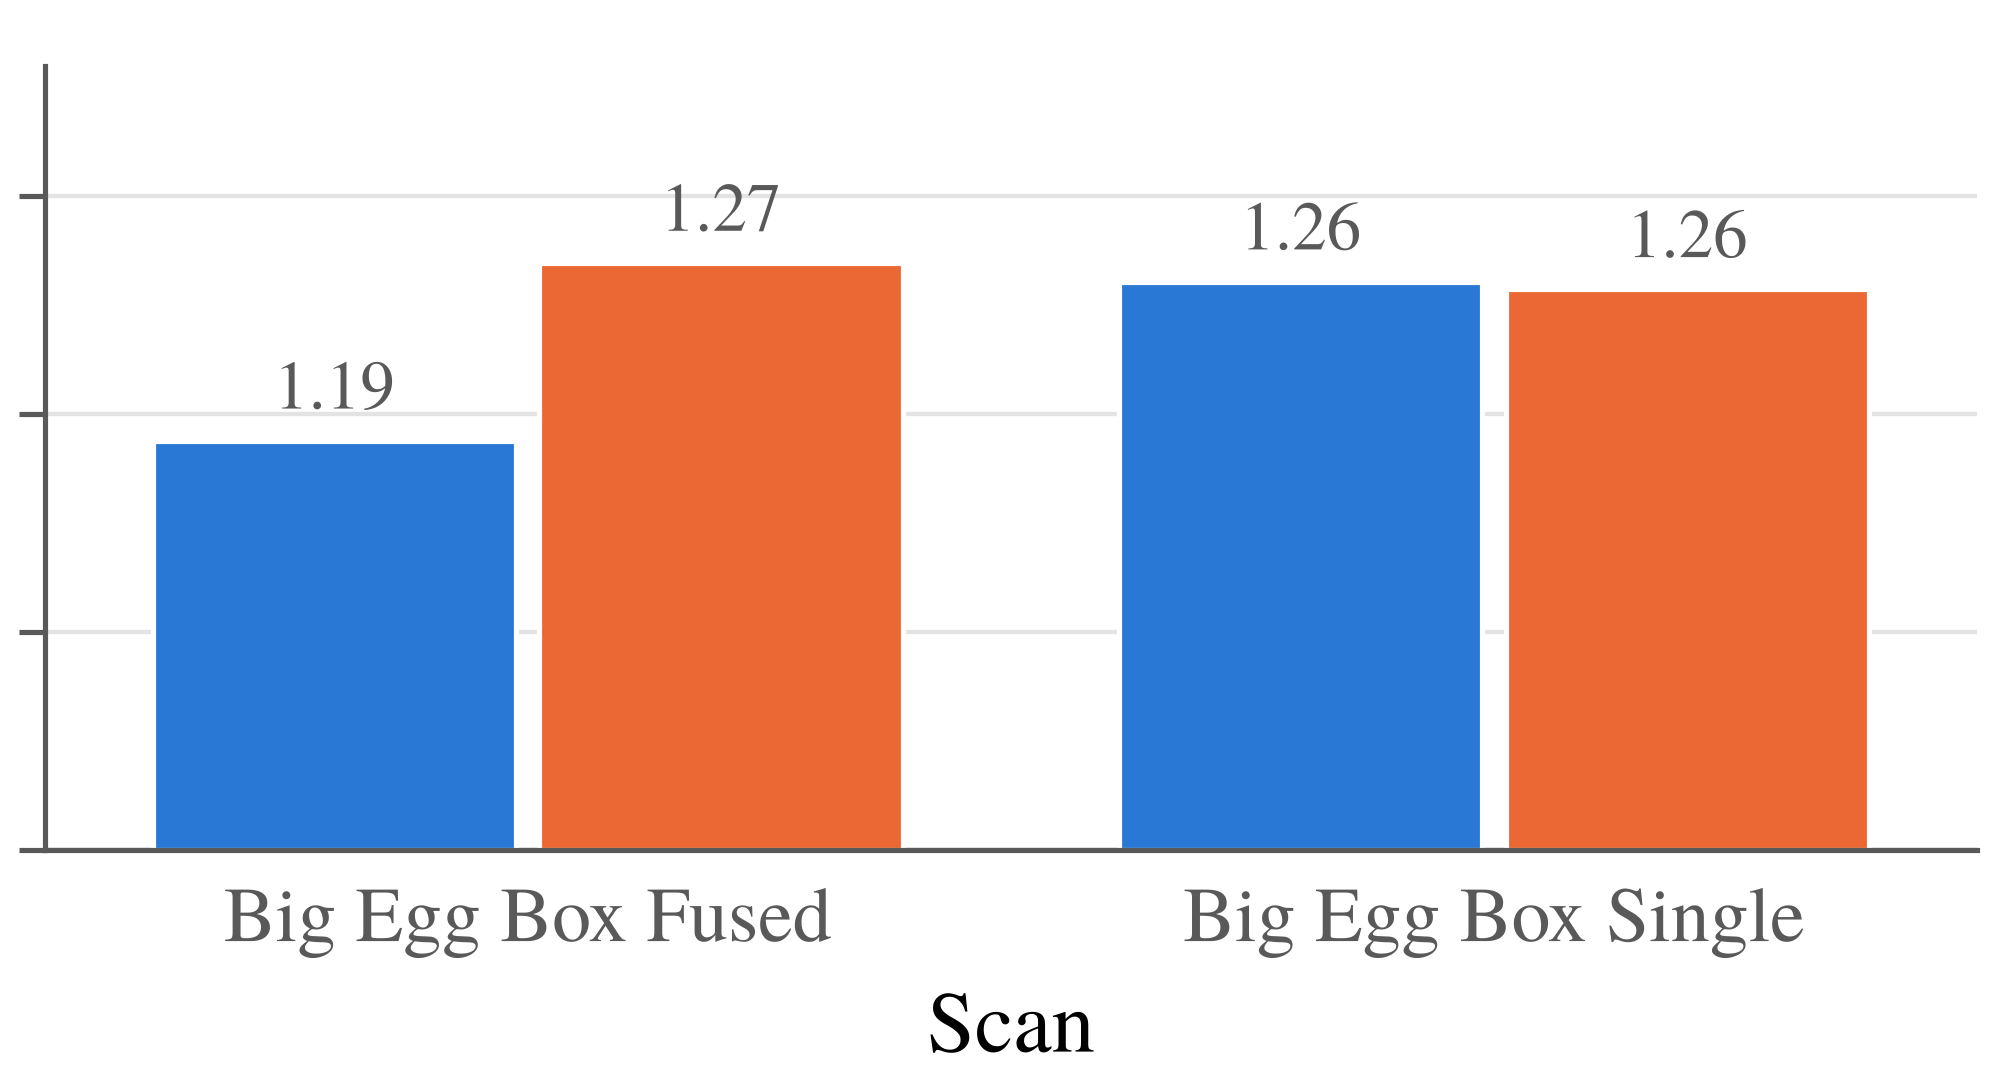
\includegraphics[width=\linewidth]{figs/ch7/Shaped/Big_Egg_Rugosity_p4}
		\caption{quartic}
		\label{fig:Big-Egg-Rugosity-4}
	\end{subfigure}
	\par\medskip
	
\includegraphics{figs/ch7/Shaped/Big_Egg_Rugosity_legend}
	\caption{Mean $\pm$ SD of n = 1 rows per bar.}
	\label{fig:Big-Egg-Rugosity}
\end{figure}

\begin{figure}[htbp]
	\centering
	\begin{subfigure}[t]{0.5072\textwidth}
		\centering
		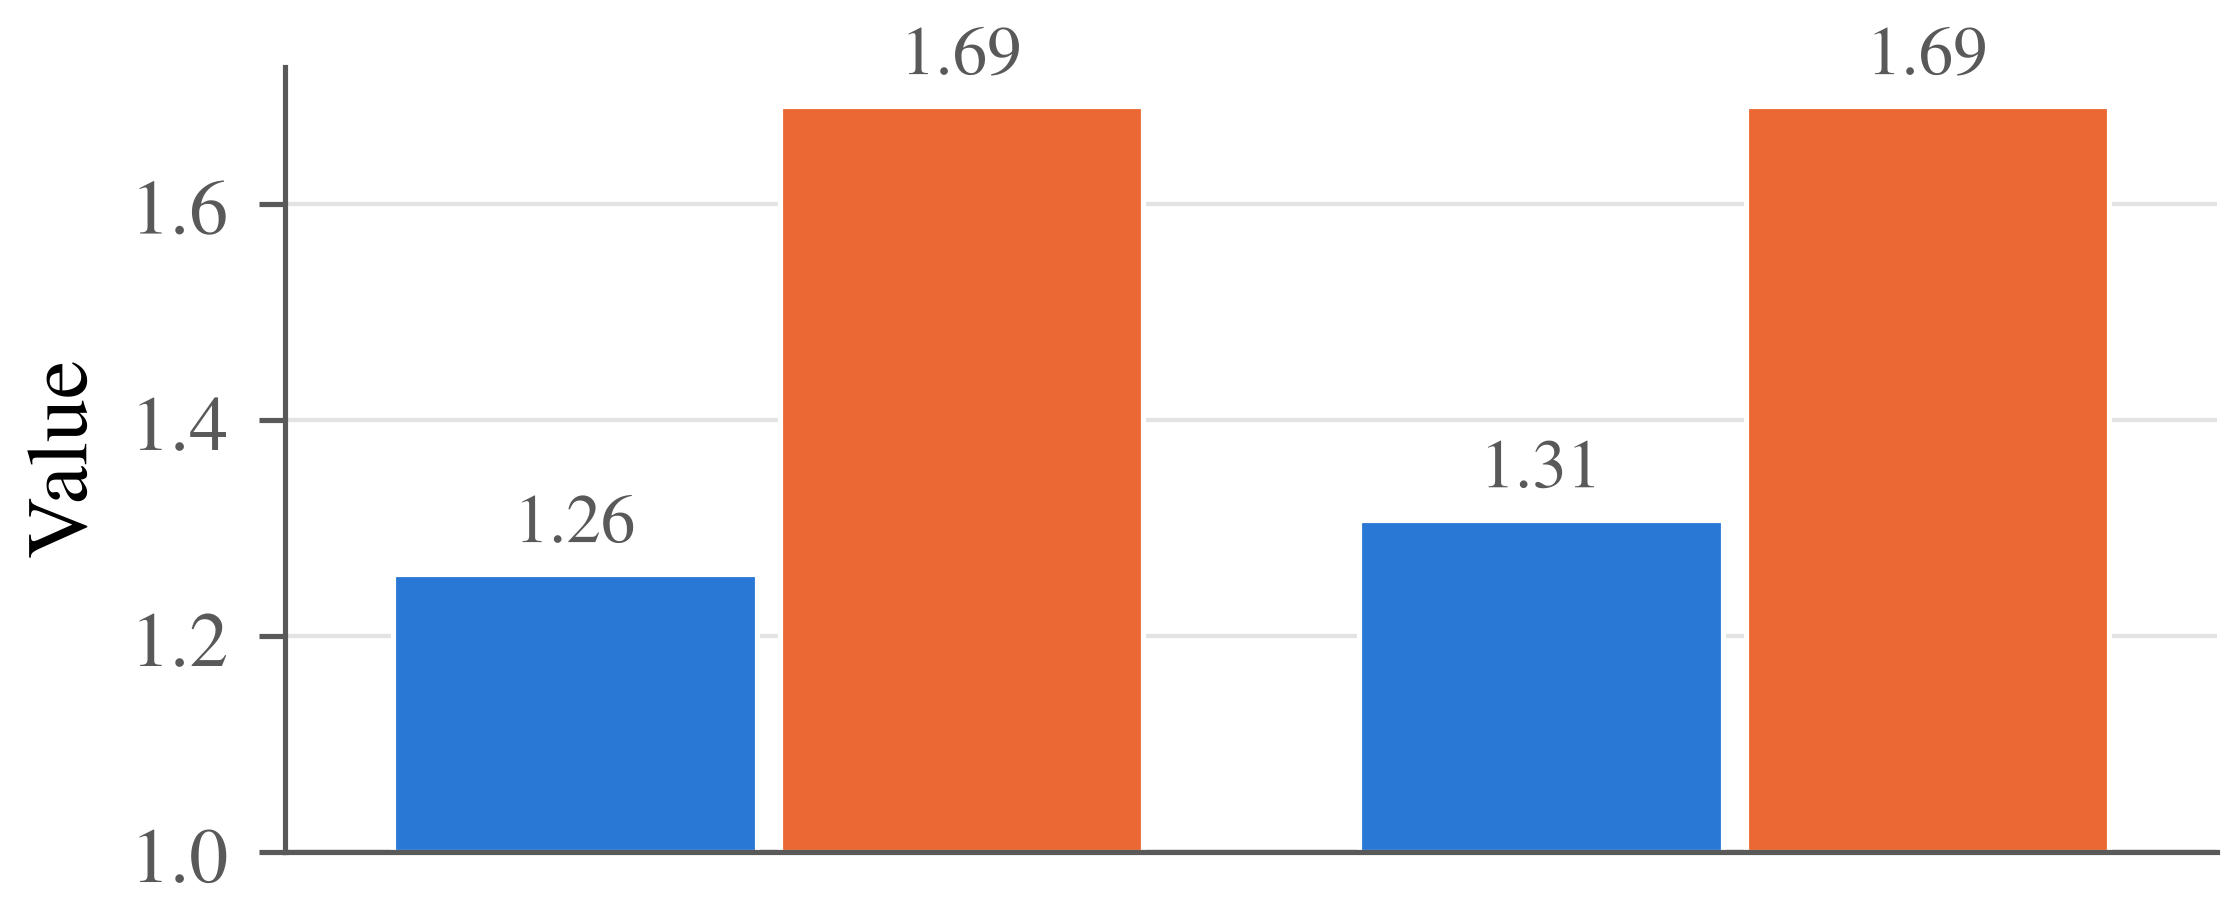
\includegraphics[width=\linewidth]{figs/ch7/Shaped/Small_Egg_Rugosity_p1}
		\caption{cubic}
		\label{fig:Small-Egg-Rugosity-1}
	\end{subfigure}\hfill
	\begin{subfigure}[t]{0.4528\textwidth}
		\centering
		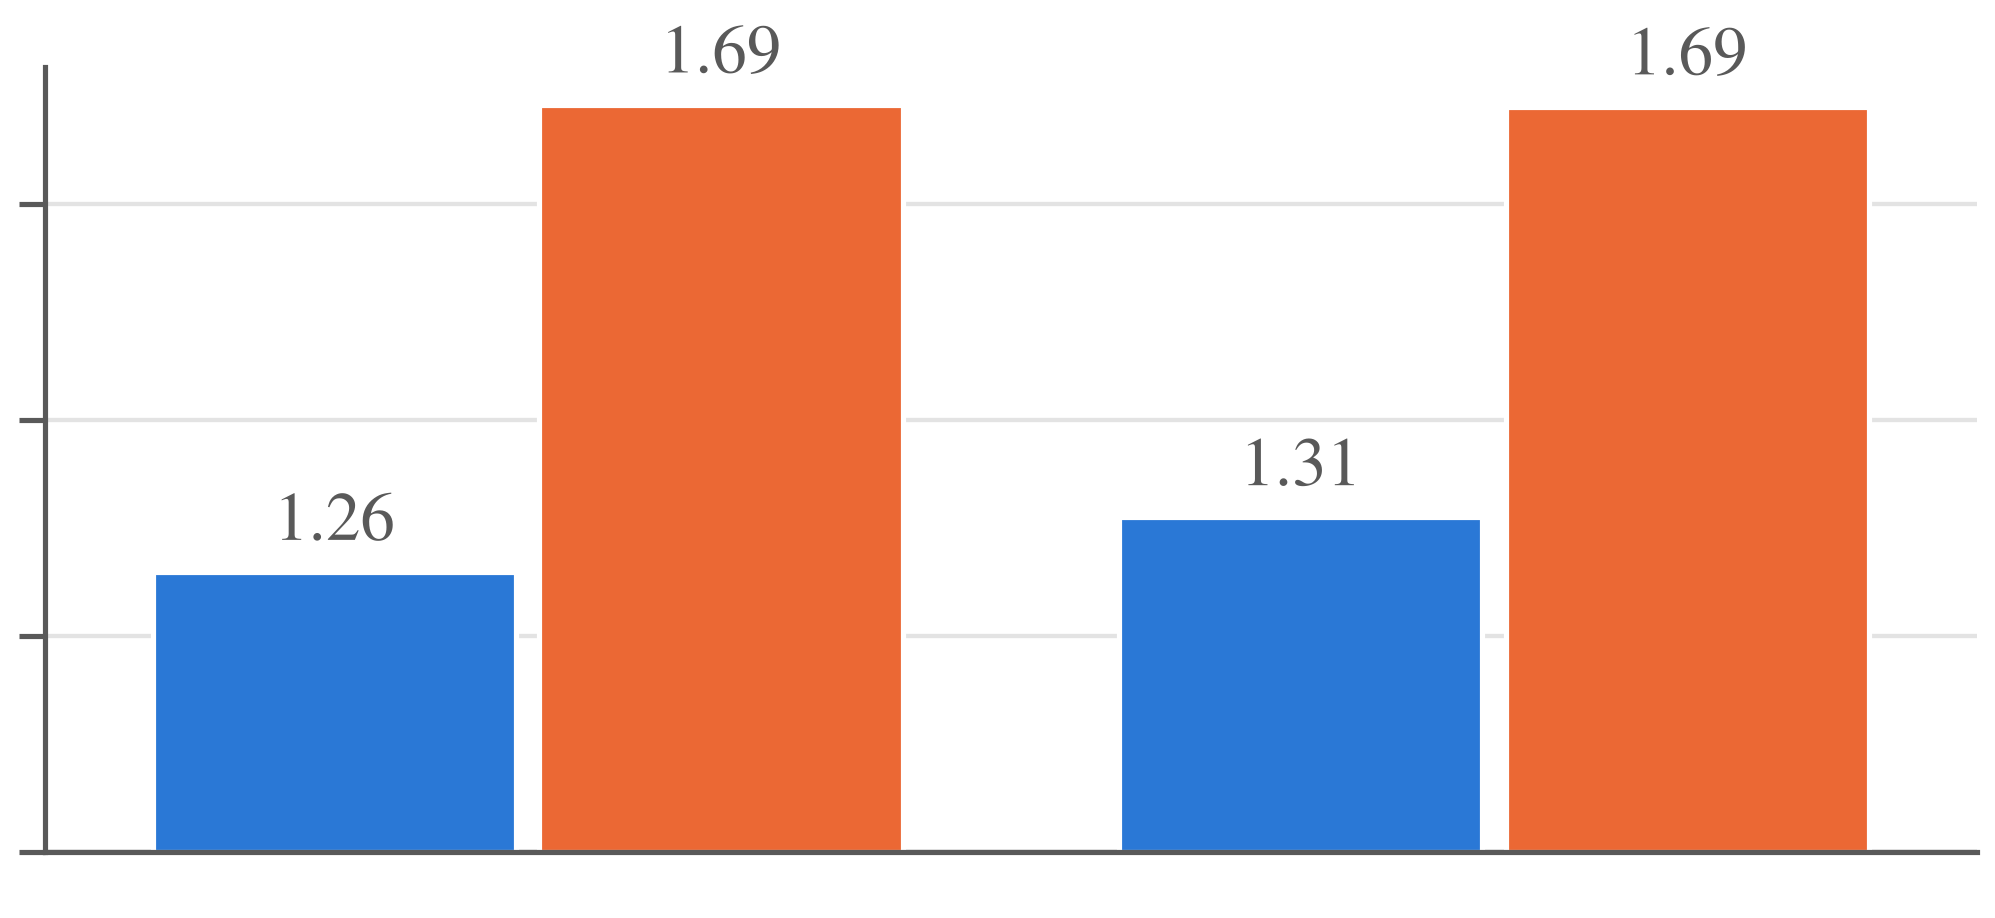
\includegraphics[width=\linewidth]{figs/ch7/Shaped/Small_Egg_Rugosity_p2}
		\caption{planar}
		\label{fig:Small-Egg-Rugosity-2}
	\end{subfigure}
	\par\medskip
	\begin{subfigure}[t]{0.5072\textwidth}
		\centering
		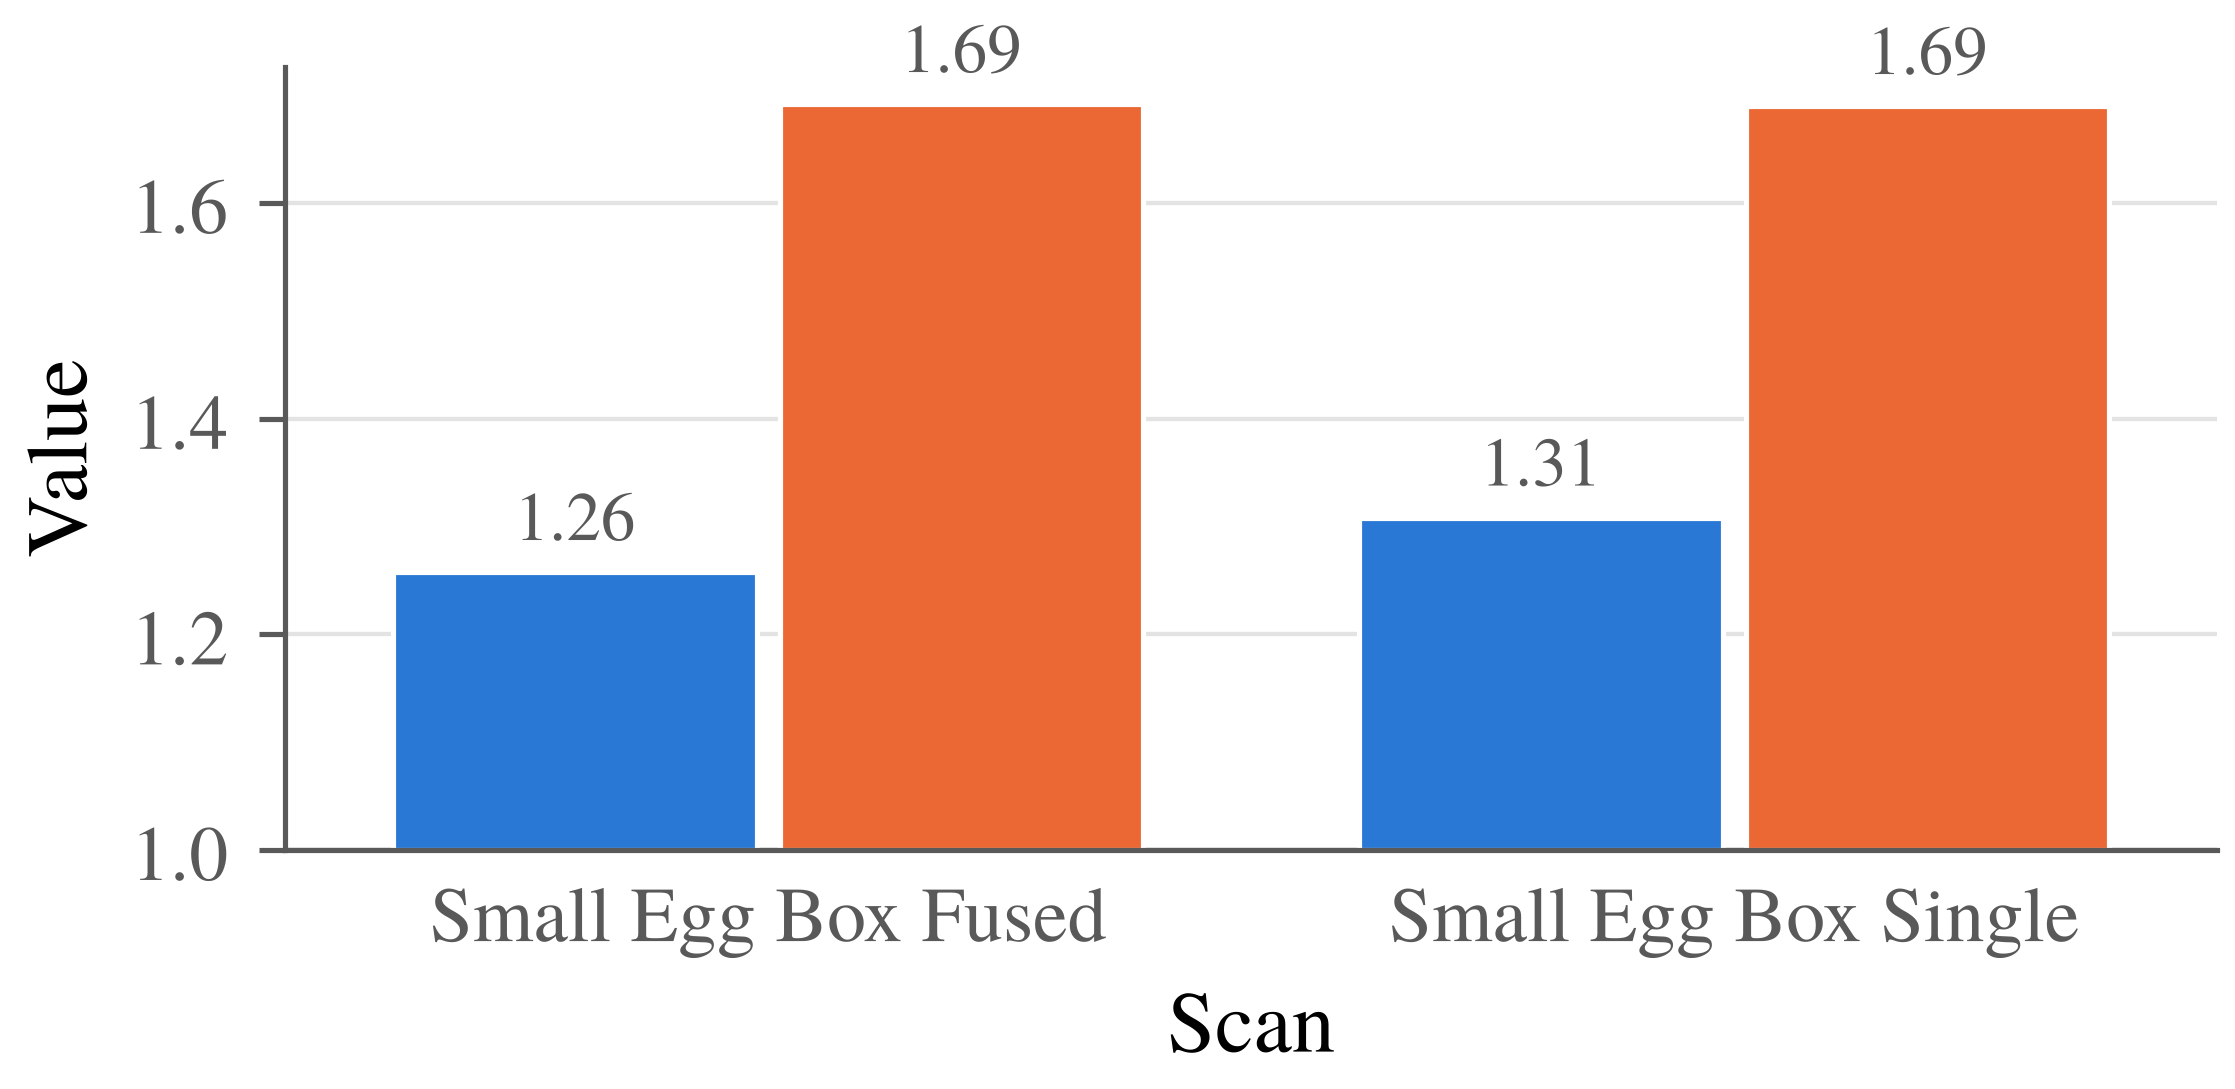
\includegraphics[width=\linewidth]{figs/ch7/Shaped/Small_Egg_Rugosity_p3}
		\caption{quadratic}
		\label{fig:Small-Egg-Rugosity-3}
	\end{subfigure}\hfill
	\begin{subfigure}[t]{0.4528\textwidth}
		\centering
		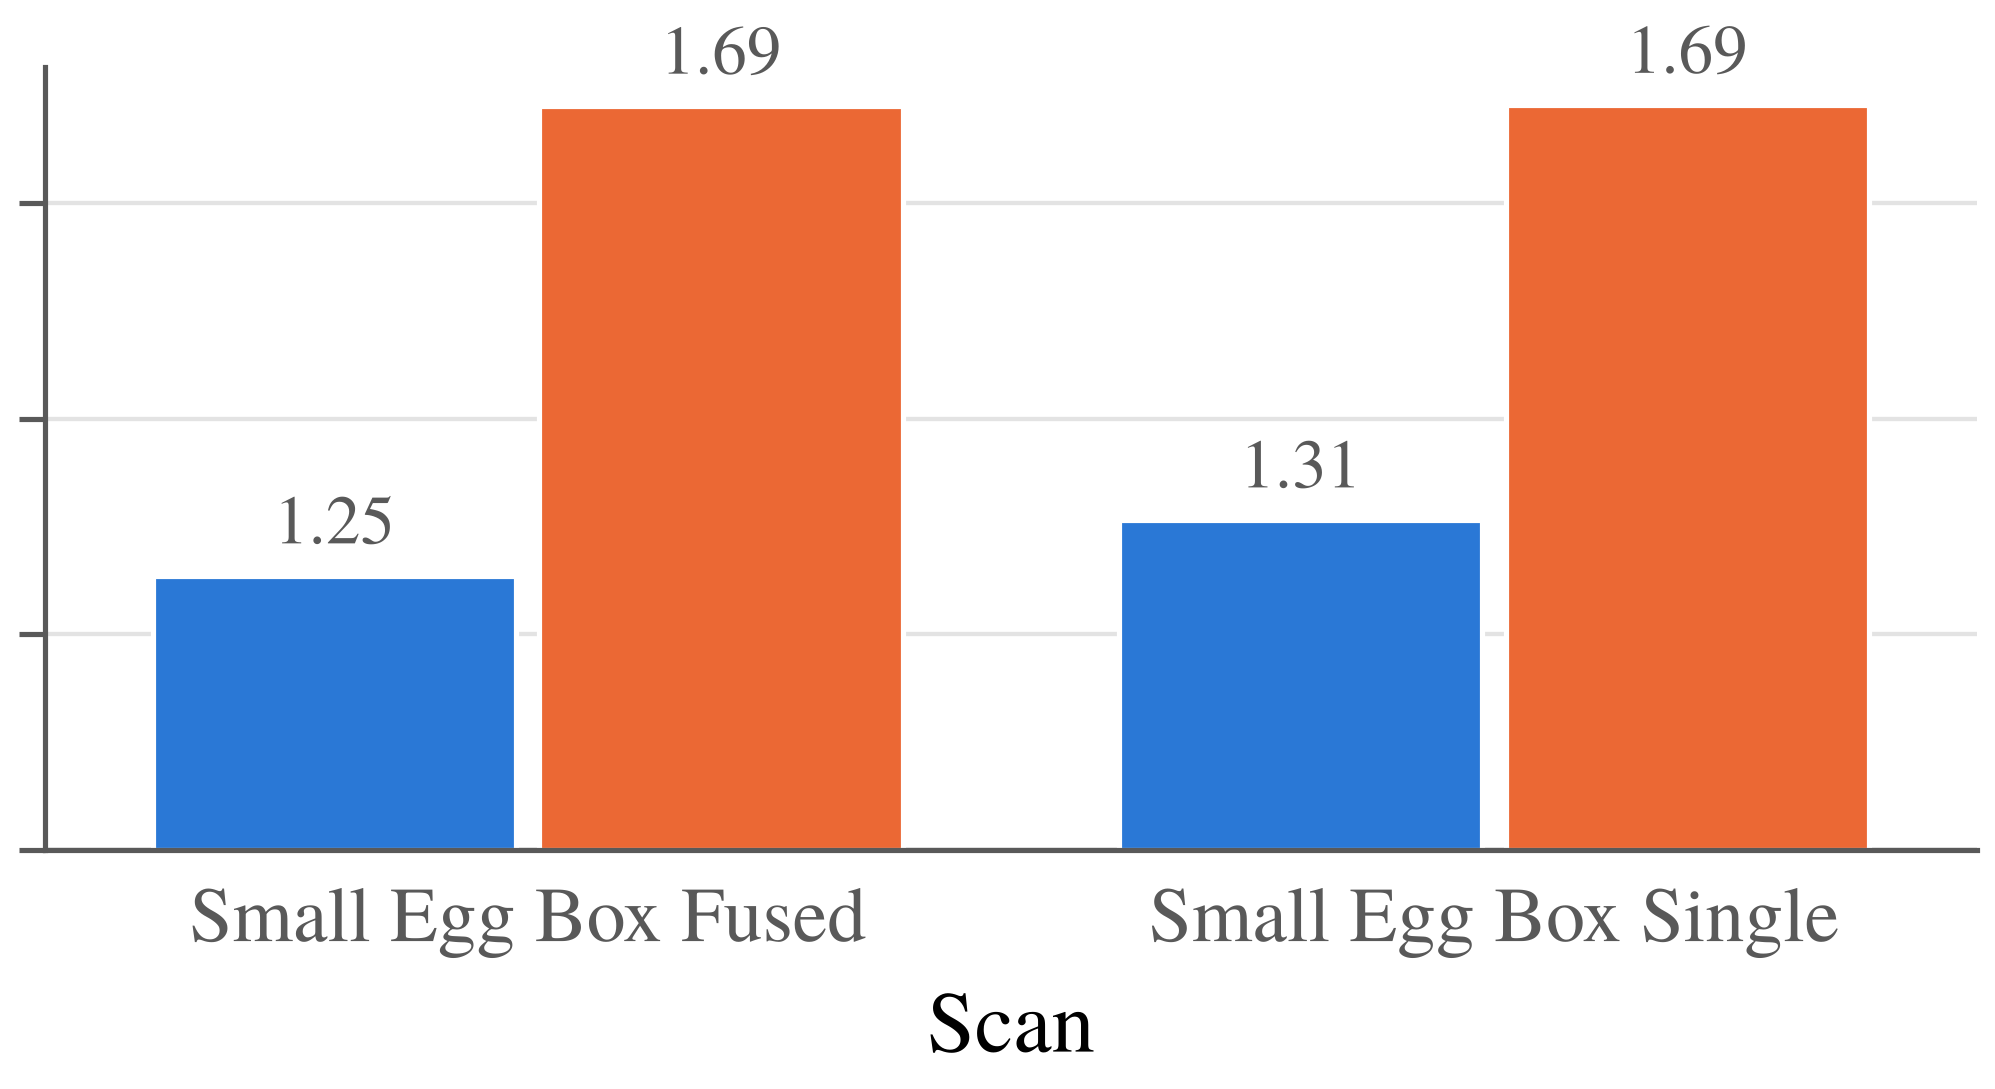
\includegraphics[width=\linewidth]{figs/ch7/Shaped/Small_Egg_Rugosity_p4}
		\caption{quartic}
		\label{fig:Small-Egg-Rugosity-4}
	\end{subfigure}
	\par\medskip
	
\includegraphics{figs/ch7/Shaped/Small_Egg_Rugosity_legend}
	\caption{Mean $\pm$ SD of n = 1 rows per bar. Fixed: Grid nx = 45.}
	\label{fig:Small-Egg-Rugosity}
\end{figure}

\section{Controlled Laboratory Sand}
\comment{Brining the Beach to the Lab
}
Whilst this reference object comparison provides an analytical evaluation, it does not align with real world conditions. Due to time constraints, real world implementation was not able to be performed, however a more realistic scan was taken, using sand collected from the langebaan lagoon. 
Approximately 13~kg of sand was collected dry, and was placed in a a 10~l plastic container. This was then flattened to produce a surface that should give rugosity metrics of 1. next, the sand was indented with the known reference shapes, and scans were taken. Next the sand was wetted with  2~kg of water. This approximates the wet intertidal sediment. The sand was then flattened again for scans, and then indented with the known reference shapes. 

Finally, for purely qualitative performance, slightly more water was added, enough to produce pools of water on the surface. The sand was then shaped by hand to have some approximate natural texture. This was then scanned. This mainly gives an estimation of the performance on more water logged regions of the sediment, and also gives an estimate on what rugosity measurements would look.

\subsection{Results}

These results show a much better trend in the performance of the system. As can be seen in the dry flat analysis, the fused scan results in a rugosity of 1.00340, which is lower than that of the unfused scan which gives a rugosity of 1.01933. This is primarily due to the fact that single scans have a higher depth noise, and on flat planar surfaces, this raises the rugosity beyond the actual natural sediment. This is what is expected, and provdes a better representation than the referenc object validation.

Unfortunately these results dont have ground truth, since they were taken from sediment that was manually flattened and shaped. However te results do show that planar surfaces result in rugosirt that is far closer to 1 than shaped surfaces, which is expected since a flat surface would result in a rugosity of exactly 1.

An interesesting results can be seen with the soaked scan. This scan is the most representative of what sediment in situ might represetnt, and the scans show that system is able to accurately represent sediment shape, even when partially submerged by water. Providing useful insigt to show the robusteness to saturated sediment.

antoher intereting metric can be seen with the wet planar surface. In the midle of this surface is a large region of high noise. This is atributed to high specular reflections of the ir projector on the predominatly flat surface, with a water film. This shows that performance can degrade under such dconditions where the projector pattern can be reflected directly back into the ir sensors. Therefore this shows that care must be taken to prevent such specular reflections.

% Generated by rstable 0.1.0 on 2026-10-22T23:42:40
% Figure: /home/joab/Documents/4022/Report/uct-thesis-template/figs/ch7/Sand/Sand_Rugosity.rsplot.json
% Data:   /home/joab/Documents/4022/Data/roughness_out_V2/Sand/roughness_results.csv
% Re-open: Sand_Rugosity_table.rstable.json. Needs booktabs and makecell.
\begin{table}[ht]
	\centering
	\small
	\setlength{\tabcolsep}{8pt}
	\caption{Each value is over n = 4 rows. Averaged over: Detrend (4), Primary (2), Flags (3), Str bounded (2), Detrend n coef (4), Detrend order (4) and 1 more.}
	\label{tab:Sand_Rugosity}
	\begin{tabular}{l c}
		\toprule
		Label & \makecell{Rugosity\\{\footnotesize mean $\pm$ SD}} \\
		\midrule
		Dry Flat & 1.00340 $\pm$ 0.00021 \\
		Dry Flat Single & 1.01933 $\pm$ 0.00018 \\
		Dry Shaped & 1.05806 $\pm$ 0.00037 \\
		Dry Shaped Single & 1.07912 $\pm$ 0.00036 \\
		Soaked & 1.02659 $\pm$ 0.00104 \\
		Soaked Single & 1.02922 $\pm$ 0.00077 \\
		Wet Flat & 1.00931 $\pm$ 0.00013 \\
		Wet Flat Single & 1.02429 $\pm$ 0.00014 \\
		Wet Shaped & 1.05924 $\pm$ 0.00023 \\
		Wet Shaped Single & 1.08549 $\pm$ 0.00011 \\
		\bottomrule
	\end{tabular}
\end{table}


\begin{figure}[htbp]
	\centering
	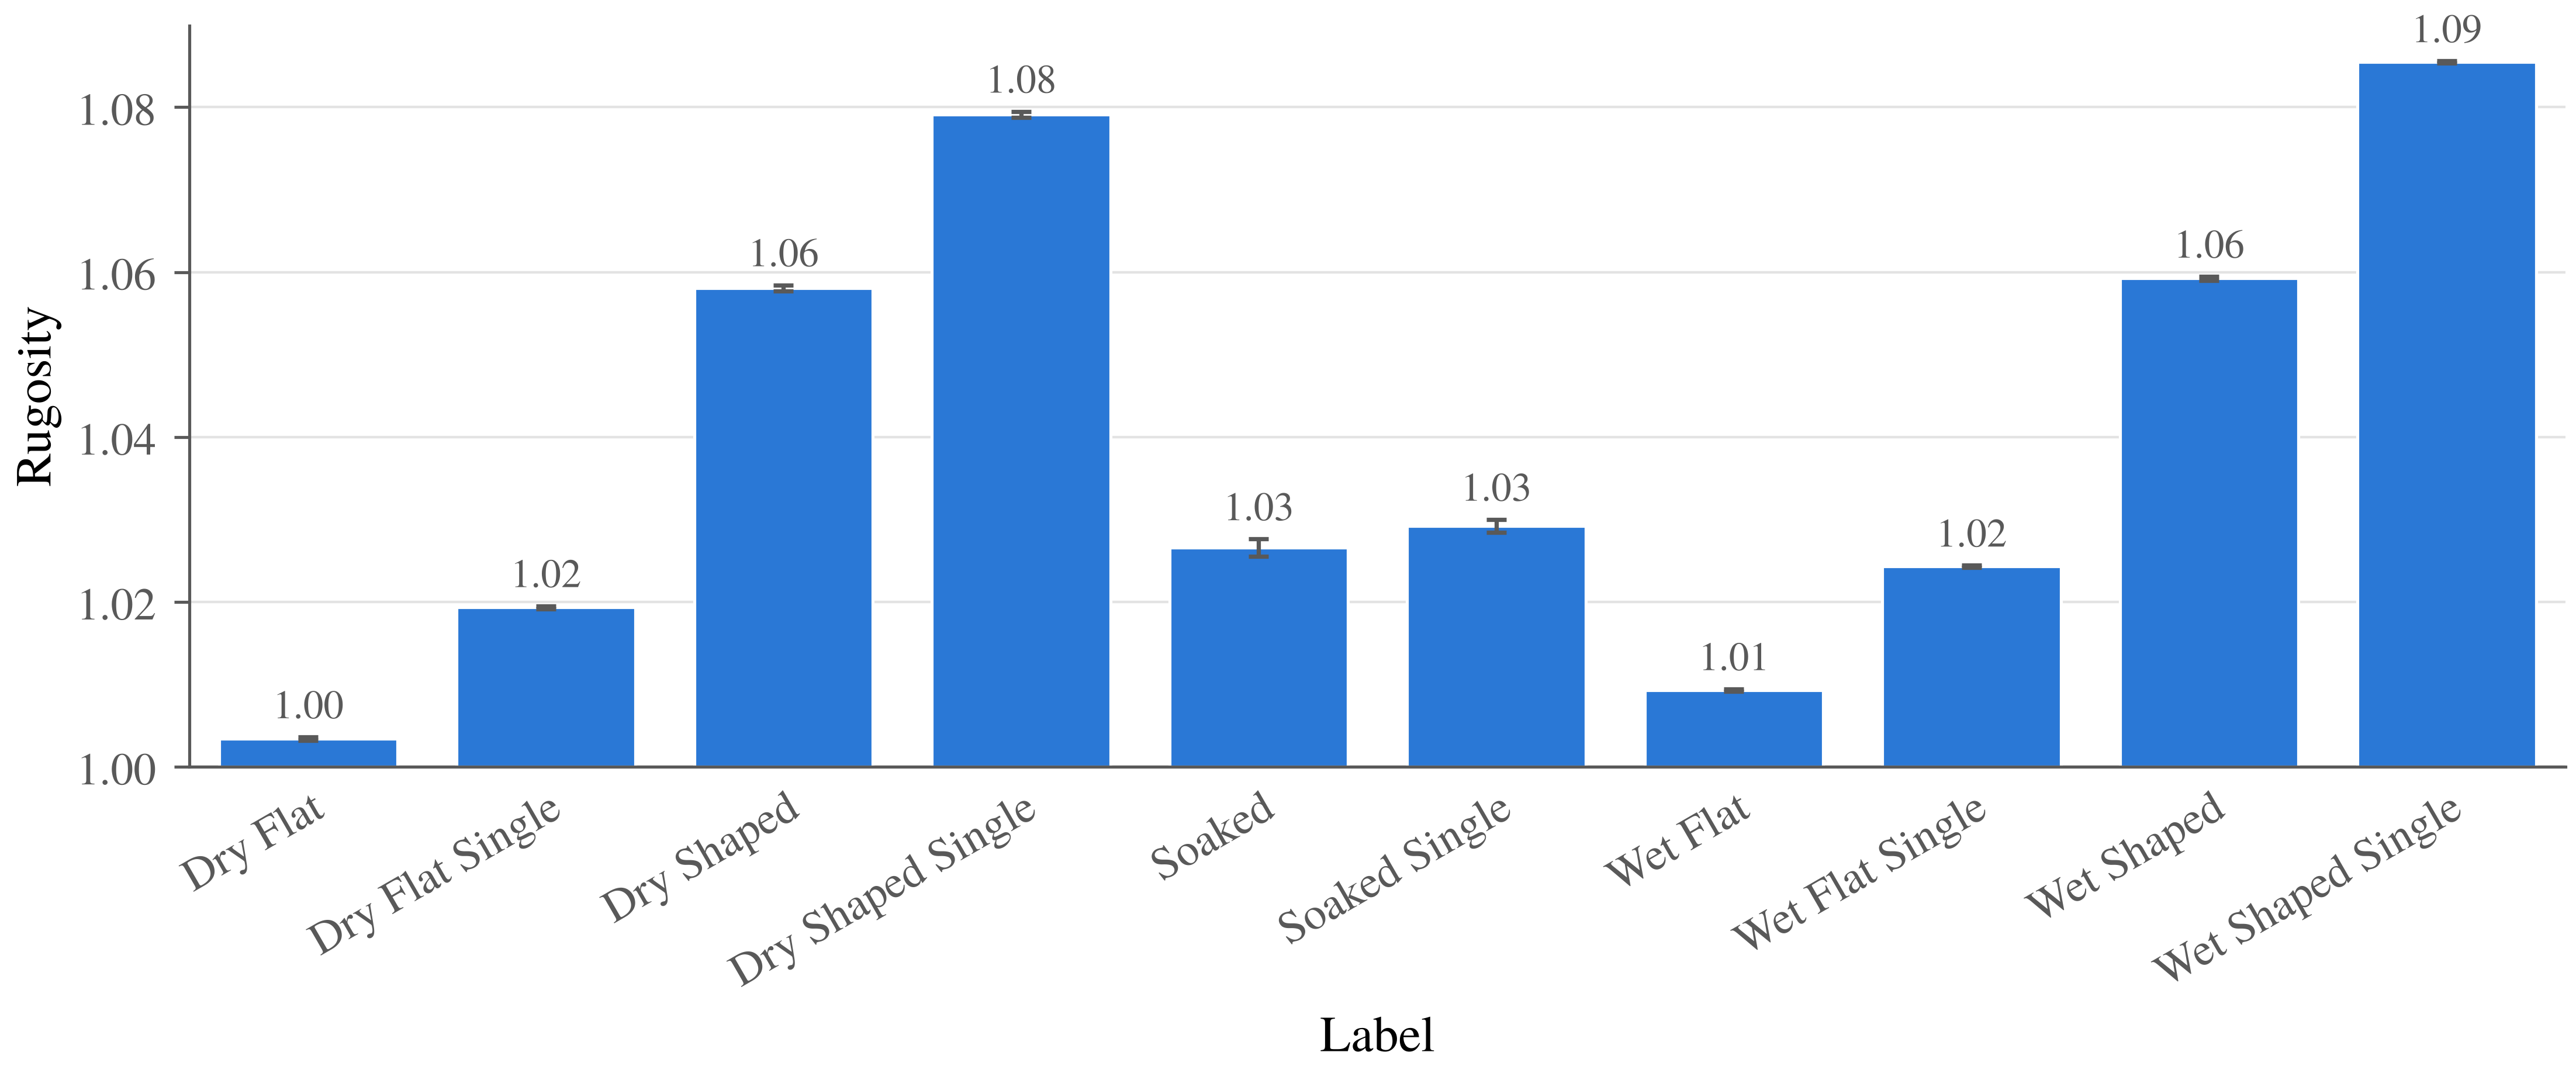
\includegraphics[width=\textwidth]{figs/ch7/Sand/Sand_Rugosity}
	\caption{Mean $\pm$ SD of n = 4 rows per bar. Averaged over: Detrend (4), Primary (2), Flags (3), Str bounded (2), Detrend n coef (4), Detrend order (4) and 1 more.}
	\label{fig:Sand-Rugosity}
\end{figure}



%*********************************************************************